% !TEX program = xelatex
\documentclass[tikz,border=0pt]{standalone}
\usepackage{fontspec}
\usepackage{xcolor}
\usetikzlibrary{calc}

\setmainfont{TeX Gyre Pagella}
\newfontfamily\sansfont{TeX Gyre Heros}

\definecolor{inknavy}{HTML}{0B1F3A}
\definecolor{tealdeep}{HTML}{164450}
\definecolor{tealmid}{HTML}{1F5A5F}
\definecolor{gold}{HTML}{C9A227}
\definecolor{goldsoft}{HTML}{E7CE7E}
\definecolor{paper}{HTML}{FAF8F3}
\definecolor{graphite}{HTML}{2A2A2A}
\definecolor{rulegray}{HTML}{D8D3C4}

\begin{document}
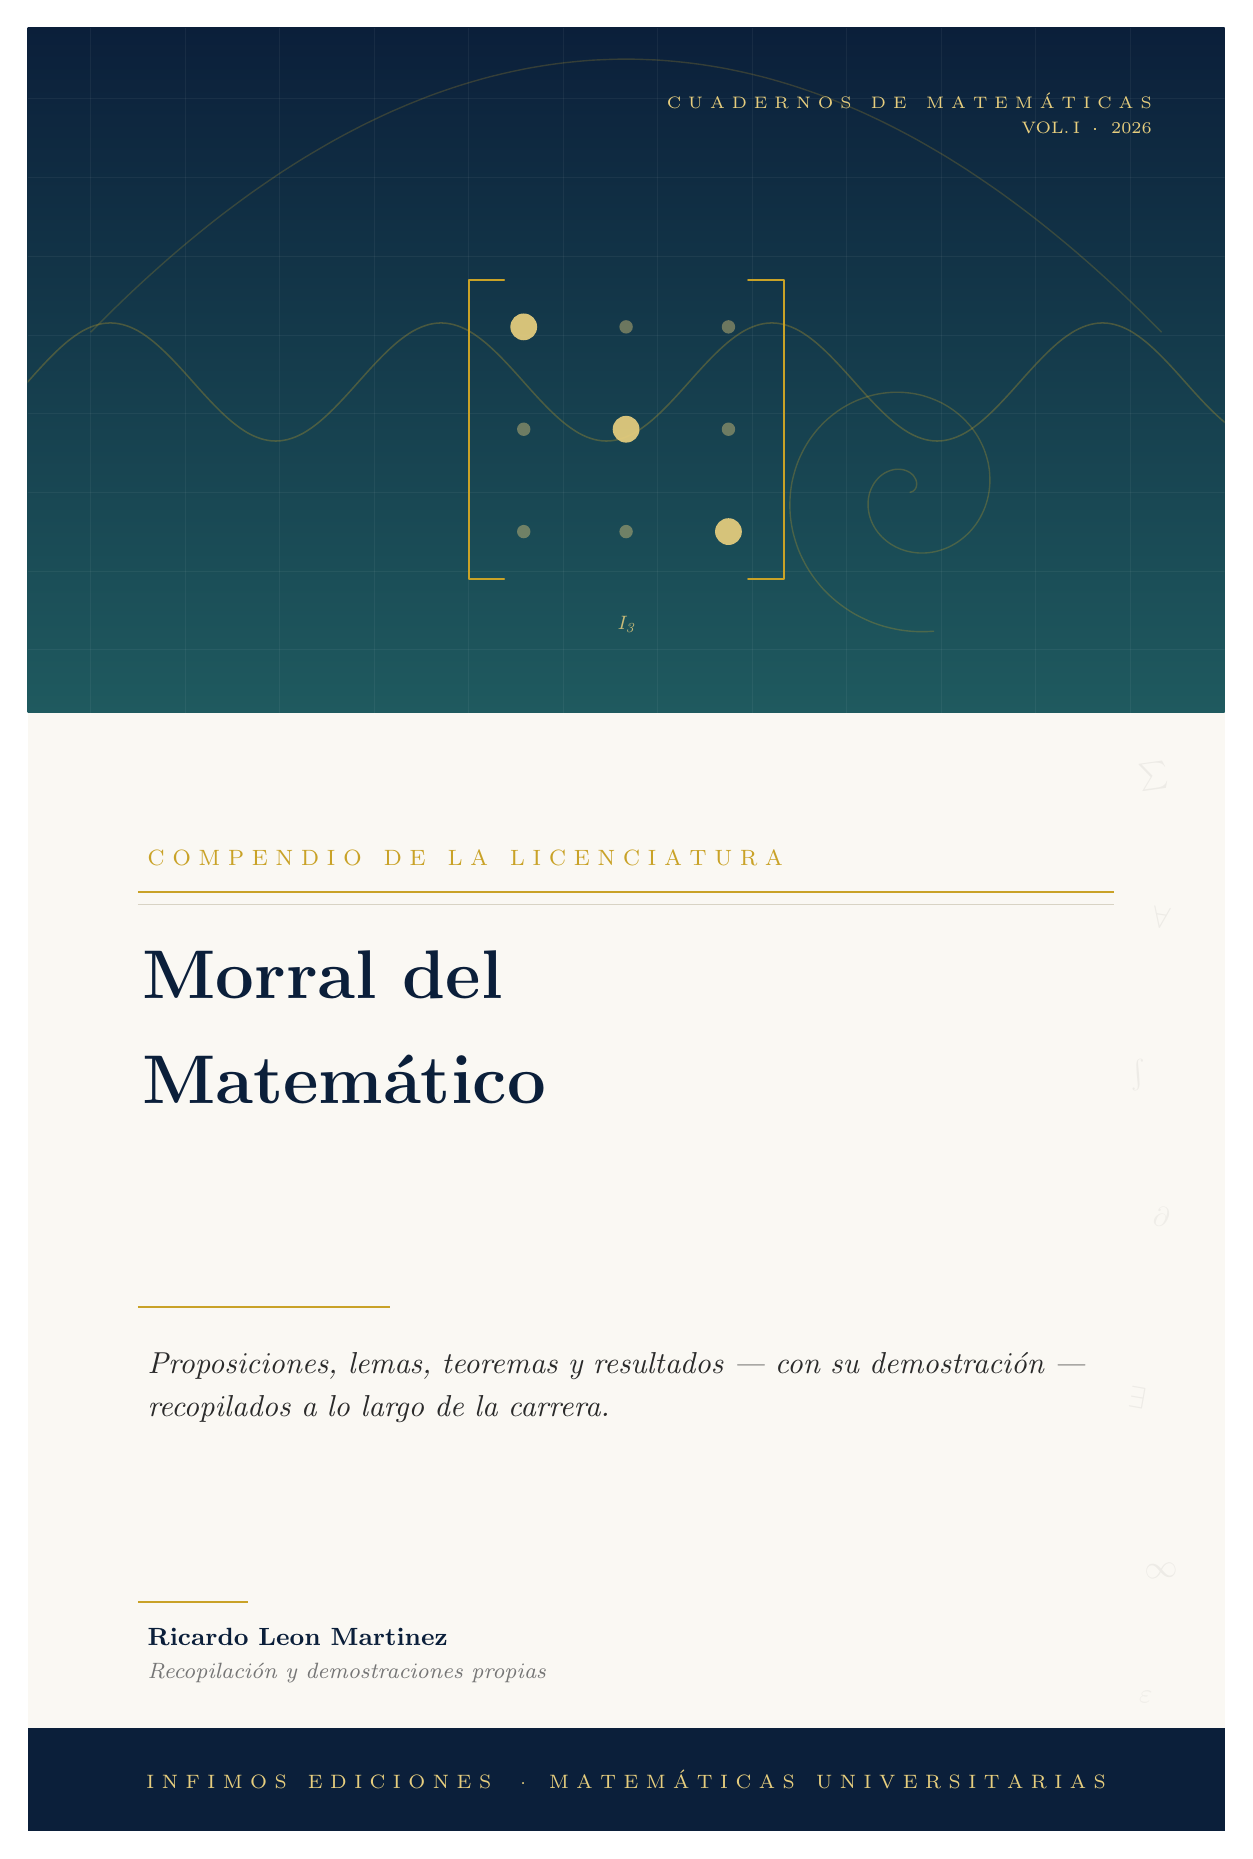
\begin{tikzpicture}[x=1mm,y=1mm]

  % ===================== FULL PAGE ======================
  \fill[paper] (0,0) rectangle (152,229);

  % ===================== IMAGE BAND (top 38%) ======================
  \begin{scope}
    \clip (0,142) rectangle (152,229);
    \shade[shading angle=115, top color=inknavy, bottom color=tealmid] (0,142) rectangle (152,229);

    % faint graph-paper grid
    \foreach \y in {150,160,...,220}{
      \draw[white,opacity=0.05,line width=0.15] (0,\y) -- (152,\y);
    }
    \foreach \x in {8,20,32,...,144}{
      \draw[white,opacity=0.05,line width=0.15] (\x,142) -- (\x,229);
    }

    % sine wave (precomputed points to avoid pgfmath dimension overflow)
    \draw[gold,opacity=0.30,line width=0.55] plot[smooth] coordinates {(-4.00,179.78) (-3.00,180.75) (-2.00,181.79) (-1.00,182.88) (0.00,184.00) (1.00,185.12) (2.00,186.21) (3.00,187.25) (4.00,188.22) (5.00,189.10) (6.00,189.86) (7.00,190.50) (8.00,190.98) (9.00,191.31) (10.00,191.48) (11.00,191.48) (12.00,191.31) (13.00,190.98) (14.00,190.50) (15.00,189.86) (16.00,189.10) (17.00,188.22) (18.00,187.25) (19.00,186.21) (20.00,185.12) (21.00,184.00) (22.00,182.88) (23.00,181.79) (24.00,180.75) (25.00,179.78) (26.00,178.90) (27.00,178.14) (28.00,177.50) (29.00,177.02) (30.00,176.69) (31.00,176.52) (32.00,176.52) (33.00,176.69) (34.00,177.02) (35.00,177.50) (36.00,178.14) (37.00,178.90) (38.00,179.78) (39.00,180.75) (40.00,181.79) (41.00,182.88) (42.00,184.00) (43.00,185.12) (44.00,186.21) (45.00,187.25) (46.00,188.22) (47.00,189.10) (48.00,189.86) (49.00,190.50) (50.00,190.98) (51.00,191.31) (52.00,191.48) (53.00,191.48) (54.00,191.31) (55.00,190.98) (56.00,190.50) (57.00,189.86) (58.00,189.10) (59.00,188.22) (60.00,187.25) (61.00,186.21) (62.00,185.12) (63.00,184.00) (64.00,182.88) (65.00,181.79) (66.00,180.75) (67.00,179.78) (68.00,178.90) (69.00,178.14) (70.00,177.50) (71.00,177.02) (72.00,176.69) (73.00,176.52) (74.00,176.52) (75.00,176.69) (76.00,177.02) (77.00,177.50) (78.00,178.14) (79.00,178.90) (80.00,179.78) (81.00,180.75) (82.00,181.79) (83.00,182.88) (84.00,184.00) (85.00,185.12) (86.00,186.21) (87.00,187.25) (88.00,188.22) (89.00,189.10) (90.00,189.86) (91.00,190.50) (92.00,190.98) (93.00,191.31) (94.00,191.48) (95.00,191.48) (96.00,191.31) (97.00,190.98) (98.00,190.50) (99.00,189.86) (100.00,189.10) (101.00,188.22) (102.00,187.25) (103.00,186.21) (104.00,185.12) (105.00,184.00) (106.00,182.88) (107.00,181.79) (108.00,180.75) (109.00,179.78) (110.00,178.90) (111.00,178.14) (112.00,177.50) (113.00,177.02) (114.00,176.69) (115.00,176.52) (116.00,176.52) (117.00,176.69) (118.00,177.02) (119.00,177.50) (120.00,178.14) (121.00,178.90) (122.00,179.78) (123.00,180.75) (124.00,181.79) (125.00,182.88) (126.00,184.00) (127.00,185.12) (128.00,186.21) (129.00,187.25) (130.00,188.22) (131.00,189.10) (132.00,189.86) (133.00,190.50) (134.00,190.98) (135.00,191.31) (136.00,191.48) (137.00,191.48) (138.00,191.31) (139.00,190.98) (140.00,190.50) (141.00,189.86) (142.00,189.10) (143.00,188.22) (144.00,187.25) (145.00,186.21) (146.00,185.12) (147.00,184.00) (148.00,182.88) (149.00,181.79) (150.00,180.75) (151.00,179.78) (152.00,178.90) (153.00,178.14) (154.00,177.50) (155.00,177.02) (156.00,176.69)};

    % gentle parabola arc
    \draw[gold,opacity=0.22,line width=0.5] plot[smooth] coordinates {(8.00,190.32) (9.36,191.69) (10.72,193.04) (12.08,194.36) (13.44,195.65) (14.80,196.91) (16.16,198.14) (17.52,199.35) (18.88,200.53) (20.24,201.68) (21.60,202.80) (22.96,203.90) (24.32,204.97) (25.68,206.01) (27.04,207.02) (28.40,208.01) (29.76,208.96) (31.12,209.89) (32.48,210.80) (33.84,211.67) (35.20,212.52) (36.56,213.33) (37.92,214.12) (39.28,214.89) (40.64,215.62) (42.00,216.33) (43.36,217.01) (44.72,217.66) (46.08,218.29) (47.44,218.88) (48.80,219.45) (50.16,219.99) (51.52,220.51) (52.88,220.99) (54.24,221.45) (55.60,221.88) (56.96,222.28) (58.32,222.66) (59.68,223.00) (61.04,223.32) (62.40,223.61) (63.76,223.88) (65.12,224.11) (66.48,224.32) (67.84,224.50) (69.20,224.65) (70.56,224.78) (71.92,224.88) (73.28,224.94) (74.64,224.99) (76.00,225.00) (77.36,224.99) (78.72,224.94) (80.08,224.88) (81.44,224.78) (82.80,224.65) (84.16,224.50) (85.52,224.32) (86.88,224.11) (88.24,223.88) (89.60,223.61) (90.96,223.32) (92.32,223.00) (93.68,222.66) (95.04,222.28) (96.40,221.88) (97.76,221.45) (99.12,220.99) (100.48,220.51) (101.84,219.99) (103.20,219.45) (104.56,218.88) (105.92,218.29) (107.28,217.66) (108.64,217.01) (110.00,216.33) (111.36,215.62) (112.72,214.89) (114.08,214.12) (115.44,213.33) (116.80,212.52) (118.16,211.67) (119.52,210.80) (120.88,209.89) (122.24,208.96) (123.60,208.01) (124.96,207.02) (126.32,206.01) (127.68,204.97) (129.04,203.90) (130.40,202.80) (131.76,201.68) (133.12,200.53) (134.48,199.35) (135.84,198.14) (137.20,196.91) (138.56,195.65) (139.92,194.36) (141.28,193.04) (142.64,191.69) (144.00,190.32)};

    % spiral (expanding), tucked to the right
    \draw[gold,opacity=0.28,line width=0.5] plot[smooth] coordinates {(112.00,170.00) (112.08,170.00) (112.16,170.02) (112.24,170.04) (112.32,170.07) (112.39,170.10) (112.47,170.15) (112.53,170.20) (112.60,170.26) (112.66,170.32) (112.71,170.40) (112.76,170.47) (112.80,170.56) (112.84,170.65) (112.86,170.74) (112.88,170.84) (112.90,170.95) (112.90,171.05) (112.90,171.16) (112.88,171.27) (112.86,171.38) (112.83,171.50) (112.79,171.61) (112.73,171.72) (112.67,171.83) (112.60,171.94) (112.53,172.05) (112.44,172.16) (112.34,172.26) (112.23,172.35) (112.12,172.44) (111.99,172.53) (111.86,172.60) (111.72,172.67) (111.57,172.74) (111.42,172.79) (111.25,172.84) (111.09,172.87) (110.91,172.90) (110.74,172.91) (110.55,172.92) (110.37,172.91) (110.18,172.90) (109.99,172.87) (109.79,172.82) (109.60,172.77) (109.41,172.70) (109.21,172.62) (109.02,172.53) (108.83,172.43) (108.65,172.31) (108.46,172.18) (108.29,172.04) (108.11,171.88) (107.95,171.71) (107.79,171.53) (107.64,171.34) (107.50,171.14) (107.37,170.92) (107.25,170.70) (107.13,170.46) (107.04,170.22) (106.95,169.97) (106.88,169.71) (106.82,169.44) (106.77,169.16) (106.74,168.88) (106.73,168.60) (106.73,168.31) (106.74,168.01) (106.78,167.71) (106.83,167.42) (106.89,167.12) (106.98,166.82) (107.08,166.52) (107.20,166.22) (107.33,165.93) (107.49,165.64) (107.66,165.36) (107.85,165.08) (108.05,164.81) (108.28,164.55) (108.51,164.30) (108.77,164.06) (109.04,163.83) (109.33,163.61) (109.63,163.41) (109.94,163.22) (110.27,163.04) (110.61,162.89) (110.96,162.74) (111.32,162.62) (111.69,162.51) (112.07,162.43) (112.46,162.36) (112.86,162.31) (113.26,162.28) (113.67,162.28) (114.08,162.29) (114.49,162.33) (114.91,162.39) (115.32,162.47) (115.74,162.58) (116.15,162.71) (116.56,162.86) (116.96,163.03) (117.36,163.23) (117.75,163.45) (118.13,163.69) (118.50,163.96) (118.86,164.24) (119.21,164.55) (119.55,164.87) (119.87,165.22) (120.17,165.59) (120.46,165.97) (120.73,166.38) (120.98,166.80) (121.20,167.23) (121.41,167.68) (121.60,168.15) (121.76,168.63) (121.90,169.12) (122.01,169.62) (122.10,170.13) (122.16,170.65) (122.20,171.17) (122.20,171.70) (122.18,172.23) (122.14,172.77) (122.06,173.30) (121.96,173.84) (121.82,174.37) (121.66,174.90) (121.47,175.43) (121.25,175.95) (121.00,176.45) (120.73,176.95) (120.42,177.44) (120.09,177.92) (119.74,178.38) (119.35,178.82) (118.95,179.25) (118.51,179.66) (118.06,180.04) (117.58,180.41) (117.08,180.75) (116.56,181.07) (116.02,181.37) (115.46,181.63) (114.88,181.87) (114.29,182.08) (113.68,182.27) (113.07,182.42) (112.44,182.54) (111.80,182.62) (111.15,182.68) (110.50,182.70) (109.85,182.69) (109.19,182.64) (108.53,182.56) (107.87,182.45) (107.21,182.30) (106.56,182.11) (105.92,181.89) (105.28,181.64) (104.65,181.35) (104.04,181.03) (103.44,180.68) (102.85,180.29) (102.29,179.87) (101.74,179.42) (101.21,178.94) (100.71,178.43) (100.22,177.89) (99.77,177.32) (99.34,176.73) (98.94,176.11) (98.57,175.47) (98.24,174.81) (97.93,174.13) (97.66,173.43) (97.43,172.71) (97.23,171.98) (97.06,171.24) (96.94,170.48) (96.85,169.71) (96.81,168.94) (96.80,168.16) (96.83,167.37) (96.90,166.59) (97.02,165.81) (97.17,165.03) (97.37,164.25) (97.61,163.48) (97.88,162.72) (98.20,161.97) (98.56,161.24) (98.95,160.52) (99.39,159.82) (99.86,159.14) (100.37,158.48) (100.91,157.84) (101.49,157.23) (102.11,156.65) (102.75,156.10) (103.43,155.58) (104.13,155.09) (104.86,154.63) (105.62,154.22) (106.41,153.84) (107.21,153.49) (108.04,153.19) (108.88,152.93) (109.74,152.72) (110.61,152.54) (111.50,152.41) (112.39,152.33) (113.29,152.29) (114.20,152.30) (115.11,152.35)};

  \end{scope}

  % ---- central emblem: matrix / linear algebra motif ----
  \begin{scope}
    \clip (0,142) rectangle (152,229);
    \coordinate (C) at (76,178);

    % bracket geometry
    \pgfmathsetmacro{\Lx}{56}   % left bracket x
    \pgfmathsetmacro{\Rx}{96}   % right bracket x
    \pgfmathsetmacro{\Ty}{197} % bracket top y
    \pgfmathsetmacro{\By}{159} % bracket bottom y
    \pgfmathsetmacro{\tick}{4.5}

    % left bracket [
    \draw[gold,line width=0.75,line cap=round,line join=round]
      (\Lx+\tick,\Ty) -- (\Lx,\Ty) -- (\Lx,\By) -- (\Lx+\tick,\By);

    % right bracket ]
    \draw[gold,line width=0.75,line cap=round,line join=round]
      (\Rx-\tick,\Ty) -- (\Rx,\Ty) -- (\Rx,\By) -- (\Rx-\tick,\By);

    % 3x3 grid of entries -- diagonal ones brighter/larger (identity matrix)
    \foreach \col/\cx in {0/63,1/76,2/89}{
      \foreach \row/\ry in {0/191,1/178,2/165}{
        \ifnum\col=\row
          \fill[goldsoft,opacity=0.92] (\cx,\ry) circle (1.7mm);
        \else
          \fill[goldsoft,opacity=0.42] (\cx,\ry) circle (0.85mm);
        \fi
      }
    }

    % tiny subscript, like a matrix dimension label
    \node[anchor=north,text=goldsoft,opacity=0.85,font=\itshape\fontsize{7}{7}\selectfont]
      at (76,155.5) {I\textsubscript{3}};
  \end{scope}

  % ---- series tag, top right ----
  \node[anchor=north east,align=right,text=goldsoft,font=\sansfont\fontsize{6.4}{8}\selectfont]
    at (144,222) {C U A D E R N O S \; D E \; M A T E M \'A T I C A S \\[1pt]
    {\fontsize{5.6}{7}\selectfont VOL.\,I \;\textperiodcentered\; 2026}};

  % ===================== FOOTER IMPRINT BAR ======================
  \fill[inknavy] (0,0) rectangle (152,13);
  \node[text=goldsoft,font=\sansfont\fontsize{6.6}{8}\selectfont] at (76,6.5)
    {I N F I M O S \; E D I C I O N E S \quad\textperiodcentered\quad M A T E M \'A T I C A S \; U N I V E R S I T A R I A S};

  % ===================== FAINT MATH TEXTURE (body) ======================
  \begin{scope}
    \clip (0,13) rectangle (152,142);
    \node[rotate=8, text=black,opacity=0.05,font=\fontsize{13}{13}\selectfont] at (143,134) {$\sum$};
    \node[rotate=-9,text=black,opacity=0.05,font=\fontsize{11}{11}\selectfont] at (144,116) {$\forall$};
    \node[rotate=10,text=black,opacity=0.05,font=\fontsize{12}{12}\selectfont] at (141,96)  {$\int$};
    \node[rotate=-6,text=black,opacity=0.045,font=\fontsize{10}{10}\selectfont] at (144,78) {$\partial$};
    \node[rotate=-10,text=black,opacity=0.05,font=\fontsize{11}{11}\selectfont] at (141,55) {$\exists$};
    \node[rotate=5, text=black,opacity=0.05,font=\fontsize{13}{13}\selectfont] at (144,33) {$\infty$};
    \node[rotate=-4,text=black,opacity=0.045,font=\fontsize{10}{10}\selectfont] at (142,17) {$\varepsilon$};
  \end{scope}

  % ===================== BODY TEXT ======================
  % eyebrow
  \node[anchor=west,text=gold,font=\sansfont\fontsize{8.2}{10}\selectfont]
    at (14,123.5) {C O M P E N D I O \; D E \; L A \; L I C E N C I A T U R A};

  % double rule under eyebrow
  \draw[gold,line width=0.55] (14,119.2) -- (138,119.2);
  \draw[rulegray,line width=0.25] (14,117.6) -- (138,117.6);

  % title
  \node[anchor=north west,text=inknavy,align=left,font=\bfseries\fontsize{31}{35}\selectfont]
    at (13.3,113) {Morral del\\[1mm] Matem\'atico};

  % small gold accent rule under title
  \draw[gold,line width=0.8] (14,66.5) -- (46,66.5);

  % subtitle
  \node[anchor=north west,text=graphite,align=left,text width=122mm,
        font=\itshape\fontsize{11.3}{15.5}\selectfont]
    at (14,62) {Proposiciones, lemas, teoremas y resultados \textemdash{} con su
    demostraci\'on \textemdash{} recopilados a lo largo de la carrera.};

  % byline
  \draw[gold,line width=0.7] (14,29) -- (28,29);
  \node[anchor=north west,text=inknavy,font=\bfseries\sansfont\fontsize{9.5}{12}\selectfont]
    at (14,27) {Ricardo Leon Martinez};
  \node[anchor=north west,text=graphite!65,font=\itshape\fontsize{8}{10}\selectfont]
    at (14,22.5) {Recopilaci\'on y demostraciones propias};

\end{tikzpicture}
\end{document}